\chapter{Obtaining Continuum Properties from $\mathcal{L}^2$-Functions}


\section{Bound and Continuum States}
Before we describe the decay of a metastable state, we have to remember,
that both bound and continuum states are involved in such a process.
Bound states are very localized and in quantum mechanics
represented by square integrable
functions of the $\mathcal{L}^2$ Hilbert space. Their boundary conditions
lead to a quantized energy spectrum and the functions of the bound states
are normalized
to represent one particle each. Unperturbed bound states are stationary
and can therefore conveniently be described using the time-independent
Schroedinger equation.
In contrast to the bound states the
continuum states are very delocalized, are not $\mathcal{L}^2$
integrable and are hence not accessible for a probabilistic interpretation.
Their energy spectrum is continuous and the functions are normalized to
their respective energy.

In decay processes
where bound and continuum states interact, it is obliged to find a way to
properly represent bound states in an energy normalization or continuum states
in an $\mathcal{L}^2$ normalization.
Since quantum chemical programme packages are based on $\mathcal{L}^2$ functions,
it is most convenient to go for the latter approach.

After an explanation of Gaussian quadrature we are going to show how
the discrete spectrum of a Hamiltonian in $\mathcal{L}^2$ representation
can be motivated to contain information of the continuum using Gaussian quadrature
based on the discussion of \cite{Reinhardt79}.
Then we are going to show, how the decay width can be obtained from a
discrete pseudo-spectrum by using Stieltjes imaging \cite{Stieltjes}.
Finally we are going to introduce the FanoADC approach for the creation of
states in the $\mathcal{L^2}$ \ac{ISR} basis.



\section{Gaussian Quadrature}
The gaussian quadrature is a numerical method for integration. By approximating
the function to be integrated $g(x) = \rho(x) f(x)$ to be a product of a
positive definite weight
function $\rho (x)$ and a continuous and bounded function $f(x)$.

The evaluation of the integral is then desired to be obtained as

\begin{equation}
  \int\limits_a^b \rho(x) f(x) dx \approx \sum\limits_{i=1}^n \omega_i f(x_i)
\end{equation}

, where the weigths $\omega_i$ and the abcissae $x_i$ are to be determined
analytically, if possible, or otherwise in an optimal way. This leads the abcissae
to be unequally spaced unlike in the basic
integration schemes using the trapezoidal rule.

The function $f(x)$ can be expressed as a polynomial.
For certain weight functions and boundaries
of integration, these
polynomials can be determined analytically.
It can furthermore be shown, that the roots (zeros) of the highest order polynomial
describing $f(x)$ give the optimal abcissae $x_i$.

In case of
$\omega(x)= \frac{1}{\sqrt{1-x^2}}$ and the condition

\begin{equation}
  \int\limits_{-1}^{1} \rho(x) Q_n(x) Q_m(x) = N_n \delta_{nm}
\end{equation}

, where $N_n$ denotes the normalization factor,
the solution to the polynomials are the so-called Chebyshev polynomials, with

\begin{equation}
  x_{i,n} = \cos \left( \frac{2i-1}{2n} \pi \right)
  \quad\quad \omega_{i,n} = \frac \pi n .
\end{equation}

\begin{figure}[ht]
  \centering
  \begin{tikzpicture}
    \begin{axis}[%scale=0.8,
                 domain=-1.0:1.0,
                 samples = 200,
                 %xtick={-3.14159,-1.57089,...,3.14159},
                 %xticklabels={$-\pi$,$-\frac \pi 2$,0,$\frac \pi 2$,$\pi$},
                 cycle list name = exotic,
                 legend style={anchor= north west},
                 legend cell align = left
                 ]
     \addplot+[domain=-1:-0.965925826289+0.135517335117/2,
              diplom1,
              mark = none,
              %forget plot,
              pattern = north east lines,
              pattern color = diplom1
              ]
              {0.0987789349866} \closedcycle;
     \addlegendentry{approximation of the integral}
     \addplot+[domain=-0.965925826289+0.135517335117/2:-0.707106781187+0.370240244847/2,
              diplom1,
              mark = none,
              forget plot,
              pattern = north east lines,
              pattern color = diplom1
              ]
              {0.646446609407} \closedcycle;
     \addplot+[domain=-0.707106781187+0.370240244847/2:-0.258819045103+0.505757579964/2,
              diplom1,
              mark = none,
              forget plot,
              pattern = north east lines,
              pattern color = diplom1
              ]
              {0.982662411472} \closedcycle;
     \addplot+[domain=-0.258819045103+0.505757579964/2:0.258819045103+0.505757579964/2,
              diplom1,
              mark = none,
              forget plot,
              pattern = north east lines,
              pattern color = diplom1
              ]
              {1.017337588535} \closedcycle;
     \addplot+[domain=0.258819045103+0.505757579964/2:0.708718898022+0.370240244847/2,
              diplom1,
              mark = none,
              forget plot,
              pattern = north east lines,
              pattern color = diplom1
              ]
              {1.353553390592} \closedcycle;
     \addplot+[domain=0.708718898022+0.370240244847/2:1.0,
              diplom1,
              mark = none,
              forget plot,
              pattern = north east lines,
              pattern color = diplom1
              ]
              {1.901221065013} \closedcycle;
     \addplot [diplom2, thick]
              {x^3 + 1};
     \addlegendentry{$f(x)= x^3 + 1$}
     %\addplot [diplom3, thick]
     %         {x^4/4 + x};
     \addplot [only marks,mark=o,thick]
       coordinates {
                   ( 0.965925826289, 1.901221065013 )
                   ( 0.707106781187, 1.353553390592 )
                   ( 0.258819045103, 1.017337588535 )
                   (-0.258819045103, 0.982662411472 )
                   (-0.707106781187, 0.646446609407 )
                   (-0.965925826289, 0.0987789349866)
                   };
     \addlegendentry{$f_i(x_i)$}
    \end{axis}
\end{tikzpicture}

  \caption{Integration by Gauss-Chebyshev quadrature of the function
           $f(x)=x^3 + 1$ (dark blue) with $n=6$. The integral (light blue)
           is approximately obtained by summation
           over all product of optimal abcissae and weights $x_if(x_i)$ (circles).}
  \label{figure:gaussian_quadrature}
\end{figure}

This means, that the integration of an arbitrary function $h(x)$ within
the interval $[-1,1]$ can be integrated as

\begin{equation}
  \int\limits_{-1}^1 h(x) dx = \int\limits_{-1}^1 \omega(x) \sqrt{1-x^2} h(x) dx
  \approx \frac \pi n \sum\limits_{i_1}^n h(x_i) \sqrt{1-x_i^2}
\end{equation}

An example for such an integration is shown in figure \ref{figure:gaussian_quadrature}
for $h(x) = x^3 + 1$. The dark blue curve shows $h(x)$, the points are the
calculated $f_i$ at the abcissae $x_i$ and the light blue hatched areas are the
approximations to the integral for the certain areas.

For an unknown weight function, the integral can be obtained by solving the so-called
moment problem.




\section{Expressing the Continuum Properties in Terms of Gaussian Quadrature}
The Hamiltonian can be expressed in terms of a complete set of eigenfunctions

\begin{equation} \label{equation:complete_hamniltonian}
  H = \sum\limits_i \ket{\phi_i} E_i \bra{\phi_i}
     + \int\limits_0^\infty \mathrm{d}E \ket{\phi(E)} E \bra{\phi(E)}  ,
\end{equation}
where the manifold of $\phi_i$ denote the bound state eigenfunctions being orthonormal
in the sense of the probabilistic picture $\braket{\phi_j|\phi_i} = \delta_{ij}$.
The continuum functions $\phi(E)$ also form an orthonormal set of basis functions
but are normalized with respect to their energy.

\begin{equation}
  \braket{\phi(E) | \phi(E')} = \delta(E-E')
\end{equation}

In a calculation using a finite $\mathcal{L}^2$ basis, the diagonalization of the
Hamiltonian yields an approximative set of eigenfunctions $\chi_i$ with corresponding
eigenvalues $\tilde{E}_i$ such that

\begin{equation}
  \tilde{H} \ket{\chi_i} = \tilde{E}_i \ket{\chi_i} \quad\quad  \,
  \braket{\chi_j|\chi_i} = \delta_{ij} .
\end{equation}

If we now rewrite the approximative Hamiltonian in terms of these $\mathcal{L}^2$
functions, we obtain

\begin{equation}
  \tilde{H} = \sum\limits_{E_i<0} \ket{\chi_i} \tilde{E}_i \bra{\chi_i}
            + \sum\limits_{E_j>0} \ket{\chi_j} \tilde{E}_j \bra{\chi_j}   ,
\end{equation}
where the first part with eigenvalues smaller than 0 corresponding to the
bound states and the second part with energies higher than 0 containing to
the continuum. In this representation the continuum is not described explicitely,
but in a discretized representation.

The eigenfunctions and eigenvalues of the positive energy solutions have no physical
meaning, because for more and more complete bases, the energies will approach zero
and the eigenfunctions will be arbitrarily diffuse. Still, they inhibit a useful
mathematical meaning if the continuum part is interpreted in terms of
a numerical quadrature.
In the case of integrating the continuum part of equation
\ref{equation:complete_hamniltonian} for evaluation of the energy expectation
value $\braket{\Psi| H | \Psi}$
with first gaussian quadrature and second the discrete positive energy
eigenfunctions, the continuum part of the expectation value reads as


\begin{align}
  \int\limits_0^\infty \mathrm{d}E \braket{\Psi|\phi(E)} E \braket{\phi(E)|\Psi}
  &\simeq \sum\limits_j \omega_j \braket{\Psi|\phi(E_j)} E_j \braket{\phi(E_j)|\Psi}
\end{align}



\begin{equation}
  \int\limits_0^\infty \mathrm{d}E \braket{\Psi|\phi(E)} E \braket{\phi(E)|\Psi}
  \simeq \sum\limits_{E_j}  \braket{\Psi|\chi} \tilde{E}_j \braket{\chi|\Psi}   .
\end{equation}

In both cases, the integral is approximated by a sum and in some special cases, where
the analytic continuum functions are known, it can be shown from the results,
that there seems to be a one-to-one corespondence between each $\mathcal{L}^2$
eigenfunction of the positive energy part and the continuum function evaluated
at the energy $\tilde{E}_j$. The equivalent quadrature weight connects the discrete and
the continuum function for the given energy and acts by renormalization.

\begin{equation}
  \ket{\chi_j} = \sqrt{\omega_j^{Eq}} \ket{\phi(\tilde{E}_j)}
\end{equation}

In the following, we are going to assume, that this equivalence between $\mathcal{L}^2$
and continuum functions with the integral interpreted as Gaussian quadrature
is true for all our systems under investigation.

If we for a moment assume, that we knew the appropriate equivalent quadrature
weigths, we could calculate the decay width from a continuous representation as

\begin{equation}
  \Gamma = \frac 1{\omega_{j}^{Eq}} \left| \braket{\Phi_s|H-E|\chi_j} \right|^2
\end{equation}

Since unfortunately in most cases, the weigth function is unknown, we are going
to calculate the weigth function by solving the moment problem, since the moments

\begin{equation}
  \Gamma^k = 2\pi \sum\limits_i \left| \braket{ \Psi | H-E | \chi_i } \right| ^2
\end{equation}
of the discrete representation are well defined and accessible,
with $\Psi$ being the wave function of the initial state.



\subsection{Moment Problem}

The moments $S(k)$ of a real and continuous function $f(\omega)$ are defined
as

\begin{equation}
  S(k) = \int\limits_a^b \omega^k f(\omega) d\omega \quad\quad k=0,1,\dots  .
\end{equation}

In case of $f(\omega)$ being a probability density function, it is connected
to the probability distribution function $F(\omega)$ via
\begin{equation}
  F(\omega) = f(\omega){d\omega} .
\end{equation}

The probability density function is completely determined by the manifold
of moments. Therefore, when all moments are known, the probability density
function  (weight function) can be calculated from the moments.
In the present case $f(\omega)$
is the decay width $\Gamma(E)$, but the theory is also applicable and very often
used for the description of cross sections. Its pseudo-spectrum has the same
mathematical properties as the pseuso-spectrum of the decay width. Therefore,
the knowledge obtained in the description of cross sections can be adopted to
the description for the decay widths.

In practice, all moments are never available unless the moments can be
calculated analytically. Therefore, one has to approximately solve the reduced
moment problem, since the density function is not completely defined.
In this case the $2r$ moments are

\begin{equation}
  S(k) = \int\limits_a^b \omega^k f(\omega) d\omega \quad\quad k=0,1,...,2r-1
\end{equation}

In principle the moment problem can be solved by requiring the abscissae and
weights to reproduce a minimum number of moment. Unfortunately, this determination
is ill conditioned and therfore, one expresses the moments by orthogonal
polynomials of some known weight function. In this case, then the
transformation to the polynomials is ill conditioned, but the abscissae
and weights can be obtained by a well conditioned problem. The latter approach
of so-called modeified moments has shown to be useful in the case of
properties such as the ionization
cross section and decay width.





\subsection{Finding the Gaussian Quadrature Abscissae and Weights from Modified Moments}

The procedure for the calculation of cross sections combining moment
theory and Gaussian quadrature has been investigated thoroughly. In this section
we follow the argumentation of Müller-Plathe \cite{}, from which the
\verb|stieltjes| routine has been written by Averbukh and which is used in
combination with the FanoADC implemented in Dirac.

For the ionization cross sections it has been shown, that the moment with
$k>2$ diverge and hence are useless for the evaluation of the probability
density function $f(\omega)$. Therefore the inverse moment $S(-k)$ are investigated
instead.

\begin{equation}
  S(-k) = \int\limits_a^b \left( \frac{1}{\omega} \right) ^k f(\omega) d\omega
\end{equation}

For each \emph{order of Stieltjes} $r$, a set of
Chebyshev polynomials
$Q_n (1/\omega) = \sum\limits_{i=0}^n Q_n^{i}\left( \frac{1}{\omega} \right)^{i}$,
of order $0-r$ can be assigned, using $2r-1$ moments.
They are orthogonal with respect to the weight function
to be determined $f(\omega)$.

\begin{equation}
  \int\limits_a^b Q_n(1/\omega) \, Q_m(1/\omega) f(\omega) d\omega = N_n \delta_{nm}
\end{equation}

They are normalized such, that the coefficient of the highest power polynomial
equals 1.

\begin{equation}
  N_n = \int\limits_a^b \left[ Q_n(1/\omega) \right]^2 f(\omega) d\omega
\end{equation}

Chebyshev polynomials in general can be constructed from an recursion formula
\begin{equation}
  Q_n(1/\omega) = \frac{1}{\omega - a_n} Q_{n-1}(1/\omega) - b_{n-1} Q_{n-2}(1/\omega)
\end{equation}

, so that all polynomials can be constructed if $Q_0$ and $Q_1$ are known.
From these recursion relations, expressions for the recursion coefficients
$a_n$ and $b_n$ can be obtained.

\begin{align}
  a_n     &= \frac{1}{b_0b_1\cdots b_{n-1}}
             \int (1/\omega)^n Q_{n-1}(1/\omega) f(\omega) d\omega
             - \sum\limits_{l=1}^{n-1} a_l  \label{equation:an_cont}\\
  b_{n-1} &= \frac{1}{b_0b_1\cdots b_{n-2}}
             \int (1/\omega)^{n-1} Q_{n-1}(1/\omega) f(\omega) d\omega \label{equation:bn_cont}
\end{align}

By expansion of the integral in equations \ref{equation:an_cont} and
\ref{equation:bn_cont} into a sum over moments obtained from the pseudo-spectra,
approximate expressions can be obtained for the recursion coefficients
depending on the energies $\bar{\omega}_i$, here the inverse abcissae,
and decay widths or the weights $\bar{f}_i$ of the
pseudo-spectrum.

\begin{align}
  a_n     &= \frac{1}{b_0b_1\cdots b_{n-1}}
             \sum\limits_{i=1}^N
               (1/\bar{\omega}_i)^n Q_{n-1}(1/\bar{\omega_i}) \bar{f}_i
             - \sum\limits_{l=1}^{n-1} a_l \label{equation:an_disc}\\
  b_{n-1} &= \frac{1}{b_0b_1\cdots b_{n-2}}
             \sum\limits_{i=1}^N
               (1/\bar{\omega}_i)^{n-1} Q_{n-1}(1/\bar{\omega}_i) \bar{f}_i
\end{align}

Hence the recursion relation now reads as
\begin{equation}
  Q_n(1/\bar{\omega}_i) = \frac{1}{\bar{\omega}_i - a_n} Q_{n-1}(1/\bar{\omega}_i)
                          - b_{n-1} Q_{n-2}(1/\bar{\omega}_i)
\end{equation}

with
\begin{equation}
  Q_0(1/\bar{\omega}_i) = 1 \quad\quad Q_1(1/\bar{\omega}_i) = (1/\bar{\omega}_i) - a_1
\end{equation}
as starting points of the determination of the polynomials.

As discussed above in section \ref{section:}, given the weights, the polynomials
can be calculated. In the Stieltjes imaging, starting from the polynomials
defined by the discrete pseudo-spectrum, one wants to achieve the weight function.
Also here the ideal abscissae are the roots of the highest order polynomial
for each moment $k$

\begin{equation}
  Q_n(1/\omega_i) = 0 \quad\quad i = 1,2,\dots ,n .
\end{equation}

The connection between the weights with the polynomials is given by

\begin{equation}
  f_i = \left[ \sum\limits_{m=0}^{n-1} \frac{Q_m^2(1/\omega_i)}{N_m} \right]^{-1} .
\end{equation}

In order to obtain the roots of the highest order polynomial, in principle
any programm for root detection can be used. However, the problem can
be reformulated in the means of general polynomials $R_n(1/\omega)$ connected
to the obtained Chebyshev polynomials
\begin{equation}
  Q_n(1/\omega) = (-1)^n \sqrt{N_n} R_n(1/\omega)
\end{equation}

with the recursion formulas
\begin{equation}
  (1/\omega)R_{n-1}(1/\omega) = - \sqrt{b_n}R_n(1/\omega) + a_nR_{n-1}(1/\omega)
                                - \sqrt{b_{n-1}} R_{n-2}(1/\omega)
\end{equation}
and
\begin{equation}
  (1/\omega)R_0(1/\omega) = - \sqrt{b_1}R_1(1/\omega) + a_1 R_0(1/\omega) .
\end{equation}

Now the roots can be determined of the following equation disregarding the
last vector by solving the eigenvalue problem.

\begin{equation}
 \begin{split}
 \begin{pmatrix}
a_1        & -\sqrt{b_1}&            &                &             &          \\
-\sqrt{b_1}& a_2        & -\sqrt{b_2}&                &             &          \\
           & -\sqrt{b_2}& a_3        & -\sqrt{b_3}    &             &          \\
           &            & \ddots     & \ddots         & \ddots      &          \\
           &            &            & -\sqrt{b_{n-2}}& a_{n-1}     & -\sqrt{b_{n-1}}\\
           &            &            &                & -\sqrt{b_{n-1}}& a_n   
 \end{pmatrix}
 \begin{pmatrix}
  R_0(1/\omega)\\
  R_1(1/\omega)\\
  R_2(1/\omega)\\
  \vdots\\
  R_{n-2}(1/\omega)\\
  R_{n-1}(1/\omega)
 \end{pmatrix}         \\
 = (1/\omega)
 \begin{pmatrix}
  R_0(1/\omega)\\
  R_1(1/\omega)\\
  R_2(1/\omega)\\
  \vdots\\
  R_{n-2}(1/\omega)\\
  R_{n-1}(1/\omega)
 \end{pmatrix}
 -
 \begin{pmatrix}
  0\\
  0\\
  0\\
  \vdots\\
  0\\
  -\sqrt{b_n} R_{n}(1/\omega)
 \end{pmatrix}
 \end{split}
\end{equation}

Therefore the solution is simplyfied to a matrix diagonalization
of the coefficients matrix. Its eigenvalues are the roots of the polynomial
and hence the wanted abcissae. The eigenfunctions are normalized to 1 and therefore
have to be renormalized according to

\begin{equation}
  1 = f_i \sum\limits_{m=0}^{n-1} R_m^2 (1/\omega_i) = \mathbf{u_i} \cdot \mathbf{u_i}
\end{equation}
from equation \ref{} to give

\begin{equation}
  f_i = N_0 u_{0i}^2
\end{equation}

for the weights.

\begin{equation}
  S(-k) = \sum\limits_{i=1}^n f_i (1/\omega_i)^k \quad\quad k=0,1,\dots,2n-1
\end{equation}





\subsection{Stieltjes Imaging}
Having obtained the abcissae and weights, the probability distribution function
$F(\omega)$ can be approximated. For this purpose the so-called Stieltjes imaging
is employed, where

\begin{equation}
  F^{(n)} (\omega) =
  \begin{cases}
    0                                & \omega < \omega_1\\
    \sum\limits_{j=1}^{i} f_j        & \omega_i < \omega < \omega_{i+1}\\
    \sum\limits_{j=1}^{i} f_j = S(0) & \omega_n < \omega 
  \end{cases}
\end{equation}
which is illustrated in figure \ref{figure:stieltjes_imaging} for a sixth
order stieltjes procedure using a pseudo-spectrum for the NeAr ICD in a
Stieltjes histogram.


\begin{figure}[h]
  \centering
  %NeAr at 3.42 AA, 6th order of stieltjes
\begin{tikzpicture}
    \begin{axis}[%scale=0.8,
                 domain=-1.0:1.0,
                 samples = 200,
                 %xtick={-3.14159,-1.57089,...,3.14159},
                 %xticklabels={$-\pi$,$-\frac \pi 2$,0,$\frac \pi 2$,$\pi$},
                 cycle list name = exotic,
                 legend style={anchor= north west},
                 legend cell align = left,
                 xlabel= {$E$ [a.u.]},
                 ylabel= {$F(E)$}
                 ]
     \addplot+[domain=-1:-0.42789448546292908,
              diplom1,
              mark = none,
%              forget plot,
              pattern = north east lines,
              pattern color = diplom1
              ]
              {0.0} \closedcycle;
     \addlegendentry{$\sum\limits_{j=1}^{i} f_j \quad \omega_i < \omega < \omega_{i+1}$}
     \addlegendimage{empty legend}
     \addlegendentry{}
     \addplot+[domain=-0.42789448546292908:-0.25969072398345394,
              diplom1,
              mark = none,
              forget plot,
              pattern = north east lines,
              pattern color = diplom1
              ]
              {0.000790314507333} \closedcycle;
     \addplot+[domain=-0.25969072398345394:0.11385089684626037,
              diplom1,
              mark = none,
              forget plot,
              pattern = north east lines,
              pattern color = diplom1
              ]
              {0.00156501308103} \closedcycle;
     \addplot+[domain=0.11385089684626037:1.4305018410002852,
              diplom1,
              mark = none,
              forget plot,
              pattern = north east lines,
              pattern color = diplom1
              ]
              {0.00208878898366} \closedcycle;
     \addplot+[domain=1.4305018410002852:5.1882229137192883,
              diplom1,
              mark = none,
              forget plot,
              pattern = north east lines,
              pattern color = diplom1
              ]
              {0.0022929712885} \closedcycle;
     \addplot+[domain=5.1882229137192883:6,
              diplom1,
              mark = none,
              forget plot,
              pattern = north east lines,
              pattern color = diplom1
              ]
              {0.00241086375443} \closedcycle;
%     \addplot [diplom2, thick,
%               domain=-0.5:6]
%              %{0.001300 * ln(x+2.594992)};
%              {0.001049 * sqrt(x+1.374436)};
%     \addlegendentry{$F(x)= \frac 13 x^3 + x^2 + 2x$}
     \addplot [samples=200,mark=*,thick,smooth,diplom2]
       coordinates {
                   (-0.42789448546292908, 0.0003951572536665)
                   (-0.25969072398345394, 0.0011776637941815)
                   ( 0.11385089684626037, 0.001826901032345)
                   ( 1.4305018410002852, 0.00219088013608)
                   ( 5.1882229137192883, 0.002351917521465)
                   };
     \addlegendentry{$\approx F(E_i)$}
    \end{axis}
\end{tikzpicture}

  \caption{Stieltjes histogram of a sixth order integration from
           an NeAr ICD pseudo-spectrum (light blue). At the abcissae $\omega_i$,
           the histogram provides lower and upper bounds for the actual
           values. The mean of these two bounds (dark blue) normally is a good
           approximation of the distribution function $F(E)$ at this point.}
  \label{figure:stieltjes_imaging}
\end{figure}

This procedure is based on the so-called Chebyshev inequalities

\begin{equation} \label{equation:Chebyshev_inequalities}
  F^{(n)}(\omega_i - 0) \le F^{(n+1)}(\omega_i - 0) \le F(\omega_i)
  \le F^{(n+1)}(\omega_i + 0) \le F^{(n)}(\omega_i + 0).
\end{equation}

This means, that the distribution functions obtained from the Chebyshev
polynomials approaching the abcissae $\omega_i$ from below and above
give lower and upper bounds to the actual value of the distribution
function at this particular point $F(\omega_i)$. In fact, the mean of these
two values normally is a very good approximation to the exact value.

\begin{equation}
  F^{(n)} (\omega_i) = \frac 12 \left[ F^{(n)} (\omega_i - 0)
                       + F^{(n)} (\omega_i+0) \right]
\end{equation}

Since we evaluated the integral,
which was the equaling quantity for both the Gaussian quadrature ansatz
in equation \ref{equation:} and the discrete spectrum in equation
\ref{equation:}, the distribution function obtained from the
discrete pseudo-spectrum is normalized correctly.
This distribution function is then numerically differenciated via

\begin{equation}
  f^{(n)} (\omega) =
  \begin{cases}
    \frac 12 \frac{f_1}{\omega_1}    & \omega < \omega_1\\
    \frac 12 \frac{f_{i+1} + f_i}{\omega_{i+1} - \omega_i}
                                     & \omega_i < \omega < \omega_{i+1}\\
    0                                & \omega_n < \omega
  \end{cases}
\end{equation}

to give  $r-1$ non-zero points of the desired
density function $f(\omega)$, which are
subsequently interpolated. In the routine of Averbukh, a spline interpolation
is used for this purpose. Afterwards the interpolated density function is evaluated
for the energy of interest, which is the resonance energy $E_r$ in case of the
autoionization processes.

\subsection{Quality and Stability of the Results}
The abcissae of the polynomials constructed from different orders
of moments intersect each other as is schematically shown in
figure \ref{figure:stieltjes_density}, where each colour of points corresponds
to one order. Therefore, in an ideal world, where all these points exactly lie
on the desired desity function, the combination of all abscissae
and weights for the interpolation is beneficial.

\begin{figure}[h]
  \centering
   \begin{tikzpicture}[
          scale=1.0,>=stealth,domain=0.5:8,samples=100,
          declare function={
          xshift = 0.7;
          yshift = 0.3;
          gamma(\x) = 1.5/(\x+xshift)^2  +yshift;
          noise(\x) = 1.5*exp(-1.0*(\x+xshift))*cos(10*(\x+xshift) r);
          calcgamma(\x) = gamma(\x) + noise(\x);
        }]
     \small
%  \draw[very thin,color=gray] (-0.1,-0.1) grid (4.9,4.9);
  \draw[->,thick] (-0.2,0) -- (5.2,0) node[right] {$E$};
  \draw[->,thick] (0,-0.2) -- (0,4.2) node[above] {$\Gamma(E)$};
  % add ticks
  \draw [thick] (4,0) -- (4,-2pt) node [anchor=north] {$E_r$};
  \draw [color=black,domain=0:5,smooth,very thick]    plot
         (\x,{gamma(\x)}) node [anchor=south east] {density function};
  \foreach \x in {0.2,0.8,...,5}
    \fill[color=orange!80] (\x,{gamma(\x)}) circle (0.08);
  \foreach \x in {0.4,1.0,...,5}
    \fill[color=diplom1!80] (\x,{gamma(\x)}) circle (0.08);
  \foreach \x in {0.6,1.2,...,5}
    \fill[color=diplom2!80] (\x,{gamma(\x)}) circle (0.08);
%  \draw [color=red,domain=0.0:5,smooth,thick]    plot
%         (\x,{calcgamma(\x)}) node [above left=20pt] {real life};
 \end{tikzpicture}
 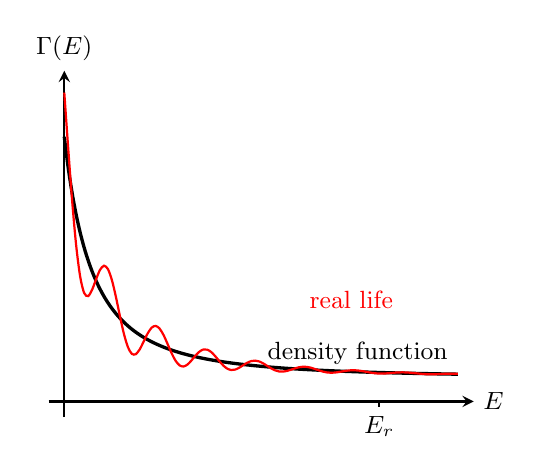
\begin{tikzpicture}[
          scale=1.0,>=stealth,domain=0.5:8,samples=100,
          declare function={
          xshift = 0.7;
          yshift = 0.3;
          gamma(\x) = 1.5/(\x+xshift)^2  +yshift;
          noise(\x) = 1.5*exp(-1.0*(\x+xshift))*cos(10*(\x+xshift) r);
          calcgamma(\x) = gamma(\x) + noise(\x);
        }]
     \small
%  \draw[very thin,color=gray] (-0.1,-0.1) grid (4.9,4.9);
  \draw[->,thick] (-0.2,0) -- (5.2,0) node[right] {$E$};
  \draw[->,thick] (0,-0.2) -- (0,4.2) node[above] {$\Gamma(E)$};
  % add ticks
  \draw [thick] (4,0) -- (4,-2pt) node [anchor=north] {$E_r$};
  \draw [color=black,domain=0:5,smooth,very thick]    plot
         (\x,{gamma(\x)}) node [anchor=south east] {density function};
%  \foreach \x in {0.2,0.8,...,5}
%    \fill[color=orange!80] (\x,{gamma(\x)}) circle (0.08);
%  \foreach \x in {0.4,1.0,...,5}
%    \fill[color=diplom1!80] (\x,{gamma(\x)}) circle (0.08);
%  \foreach \x in {0.6,1.2,...,5}
%    \fill[color=diplom2!80] (\x,{gamma(\x)}) circle (0.08);
  \draw [color=red,domain=0.0:5,smooth,thick]    plot
         (\x,{calcgamma(\x)}) node [above left=20pt] {real life};
 \end{tikzpicture}

  \caption{Schematic illustration of the interpolation after the
           stieltjes calculations to yield the density function $\Gamma(E)$,
           which is to be evaluated at the resonance energy $E_r$.
           Suppose the black curve to be the
           exact result. Then (left panel), for each order of Stieltjes calculation
           the points lie on this curve, where points from different orders
           (different colours of the points) intersect each other. The interpolation
           gives the exact result. In reality (right panel) the
           interpolations (even of each moment)
           are likely to show oscillations due to non-orthogonalities of
           Chebyshev polynomials in the higher orders and inaccurate descriptions
           due to a large gap between the lower and upper bounds for low
           orders.}
  \label{figure:stieltjes_density}
\end{figure}

As can be seen from the Chebyshev inequalities in
equation \ref{equation:Chebyshev_inequalities}, the higher the highest
power of the polynomials and hence the larger the degrees of freedom are,
the closer the lower and upper bounds get to the exact result.

Unfortunately, the moment problem is ill-conditioned and by introducing
the polynomials, the moment problem as such get well-conditioned but instead
the construction of the polynomials from the pseudo-spectrum is ill-conditioned.
As can be seen from the Chebyshev inequalities, one would like to go to as
high orders as possible, to get more accurate results. But in the construction
of the recursion coefficients \ref{equation:an_disc}, two very large numbers
are subtracted from each other. This is known to be numerically instable.
And the higher the order of the moment is, the bigger
are these numbers and hence the introduced error. Therefore the number
of moments to be successfully employed for the approximation of the
density function is limited by the quality of the orthogonality of
the corresponding set of constructed polynomials. In the final density function
non-orthogonalities as well as errors from inaccurate descriptions of lower
orders can be detected by the presence of oscillations as shown in
figure \ref{figure:stieltjes_density} in the right panel. In case of the density
function being well behaved in the area of the resonance energy $E_r$, the
description might still be feasible. In case of strong oscillations, the validity
of the results are highly questionable. The interpolation can be smoothed
by taking only stable orders of stieltjes into account or in other words
reduce the allowed threshold of allowed non-orthogonality or to give points
stemming from lower orders of Stieltjes higher weights in the interpolation.
